\section{Creature Generation}

\subsection{Automatisches Rigging}
Um die Bone-Struktur des generierten Skelettes mit dem Mesh zu verknüpfen, muss bei der 3D-Modellierung der Prozess des Riggings durchlaufen werden. Dieser beschreibt wie sich jeder einzelne Vertex des Meshes mit den Bones in der Szene bewegt. Jeder Vertex kann an beliebig vielen Bones angehängt werden. Durch eine Gewichtung wird bestimmt wie sehr ein Vertex durch der Transformation eines Bones mitbewegt wird.
Da sowohl das Skelett, als auch das gesamte Mesh prozedural generiert werden, kann das Rigging nicht wie üblich in einem Modellierungs-Tool wie Blender~\cite{blender} manuell durchgeführt werden, sondern muss zur Laufzeit des Spiels während der Generierung der Kreaturen geschehen.

Für ein erfolgreiches Rigging ist es wichtig, dass das Skelett bereits sinnvoll in dem Mesh eingebettet ist. Da hier das Mesh aus Metaballs generiert wird, welche um die Bones plaziert sind, können wir hier davon ausgehen, dass das Mesh das Skelett bereits \emph{sinnvoll} umhüllt.

\begin{figure}[h!]
	\centering
	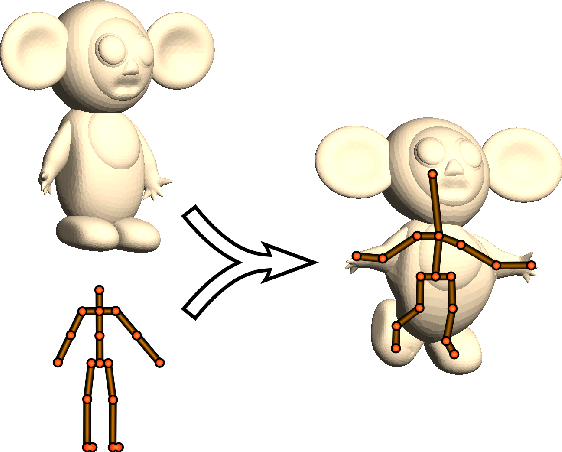
\includegraphics[width=0.6\linewidth]{resources/img/skeleton_embedding.png}
	\caption{Beispiel für ein korrekt eingebettetes Skelett in einem Mesh~\cite{bone_heat_paper}.}
	\label{fig:skeleton_embedding}
\end{figure}

Während der Entwickelung wurde zunächst eine triviale Methode als Zwischenlösung verwendet. Dabei wurden alle Vertices nur an den Bone mit der geringsten Distanz angehängt. Diese Methode ist jedoch visuell unbrauchbar, da bei Bewegung des Skeletts an den Gelenken zwischen den Bones Löcher und verschiedene andere Artefakte entstehen. Es wird also eine Lösung benötigt, die es ermöglicht Vertices an mehrere Bones anzuhängen und die Gewichte so bestimmt, dass das Mesh an den Übergängen zwischen den Bones möglichst natürlich deformiert wird.

Ein bereits bekannter Algorithmus zur automatisch Gewichtsberechnung und Verknüpfung des Meshes ist die Bone-Heat Methode~\cite{bone_heat_paper}. Dieser berücksichtig mehrere zusätzliche Eigenschaften für die Gewichte. Zuerst sollen die Gewichte unabhängig von der Auflösung des Meshes sein. Außerdem müssen die Gewichte sich sanft über den Verlauf der Oberfläche verändern. Die Breite des Übergangs zwischen zwei Bones sollte ungefähr proportional zu der Distanz des Gelenks zur Oberfläche des Meshes sein.
Ein Algorithmus, welcher die Gewichte alleine aus der Distanz der Bones zu den Vertices berechnet, kann oft schlechte Ergebnisse liefern, da er die Geometrie des Modells ignoriert. Zum Beispiel können Teile des Torsos mit einem Arm verbunden werden. Die Bone-Heat Methode behandelt stattdessen das innere Volumen des Modells als einen wärmeleitenden Körper. Es werden für jeden Vertex die Gleichgewichts-Temperatur berechnet und diese als Gewichte für die Bones verwendet. Wie in Abbildung~\ref{fig:bone_heat_equilibrium} zu sehen ist, wird ein Bone auf 1° gesetzt und der andere auf 0°. Bei Deformation der beiden Bones mit den Gewichten aus dem Temperatur-Gleichgewichts entsteht an dem Gelenk eine natürlich aussehende Verformung der Oberfläche.

\begin{figure}[h!]
	\centering
	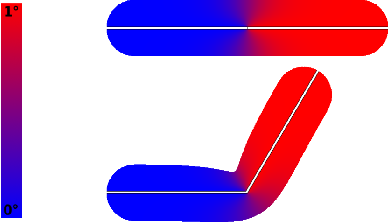
\includegraphics[width=0.7\linewidth]{resources/img/bone_heat_equilibrium.png}
	\caption{Temperatur-Gleichgewicht für zwei Bones~\cite{bone_heat_paper}.}
	\label{fig:bone_heat_equilibrium}
\end{figure}

Das Temperatur-Gleichgewicht des Volumens zu berechnen wäre sehr aufwändig und langsam, deswegen wird das Gleichgewicht nur über die Oberfläche des Meshes berechnet. Die Gewichte für Bone $i$ werden berechnet durch:

\begin{equation}
    \label{eq:bone_heat}
    \begin{aligned}
        &\frac{\partial\mathbf{w}^i}{\partial t} = \Delta\mathbf{w}^i+\mathbf{H}\left(\mathbf{p}^i-\mathbf{w}^i\right)=0 \\
        \iff &-\Delta\mathbf{w}^i+\mathbf{H}\mathbf{w}^i=\mathbf{H}\mathbf{p}^i \\
        \iff &\left(-\Delta+\mathbf{H}\right)\mathbf{w}^i=\mathbf{H}\mathbf{p}^i
    \end{aligned}
\end{equation}

Dabei ist $\Delta$ der diskrete Laplace-Beltrami Operator auf der Oberfläche des Meshes, welcher mit der Kotangens-Methode approximiert wird~\cite{laplace_beltrami_paper}. $\mathbf{p}^i$ ist ein Vektor mit $p^i_j=1$ wenn der nächste Bone zum Vertex $j$ der Bone $i$ ist. Sonst ist $p^i_j=0$. $\mathbf{H}$ ist eine Diagonalmatrix wobei $H_{jj}$ die Hitze des nächsten Bones von Vertex $j$ ist. Sei $d(j)$ die Distanz zum nächsten Bone von Vertex $j$, dann wird $H_{jj}=c/d(j)^2$ gesetzt. Allerdings nur wenn das Geradensegment von dem Vertex zu dem Bone vollständig in dem Volumen des Modells enthalten ist. Wenn der Bone von dem Vertex aus also nicht sichtbar ist, wird $H_{jj}=0$ gesetzt. Dies verhindert, dass beispielsweise Vertices am Arm and den Torso angehängt werden. Wenn mehrere Bones nahezu die gleiche Distanz zu dem Vertex haben und sichtbar sind, werden ihre Anteile an der Temperaturverteilung gleich berücksichtigt. $p_j$ wird dann $1/k$ und $H_{jj} = kc/d(j)^2$

Der benötigte Sichtbarkeits-Test wird durch ein Signed-Distance-Field (SDF) realisiert, welches wir vorab mit einem Geometry-Shader generieren. Damit werden effiziente Raycast-Operationen in dem Mesh möglich. (TODO: passendes Zitat finden)
Der Parameter $c$ wird in dem Paper~\cite{bone_heat_paper} auf $1$ gesetzt, um natürlichere Ergebnisse zu erreichen. Für $c\approx0.22$ würde der Algorithmus Gewichte berechnen die ähnlicher zu dem Temperatur-Gleichgewicht über dem tatsächlichen Volumen des Meshes sind.

Für die effiziente Lösung des Matrix-Systems~\ref{eq:bone_heat} ist es wichtig die Eigenschaften des diskreten Laplace-Beltrami Operators $\Delta$ näher zu betrachten. Der Operator wird durch die Kotangens-Methode approximiert, indem von jedem Vertex $x_i$ für jede ausgehende Kante ein Gewicht $v(x_i,x_j)$ aus den gegenüberliegenden Winkel $\alpha_{ij}$ und $\alpha_{ji}$ berechnet wird (siehe Abbildung~\ref{fig:cotangent_approx}).

\begin{figure}[h!]
	\centering
	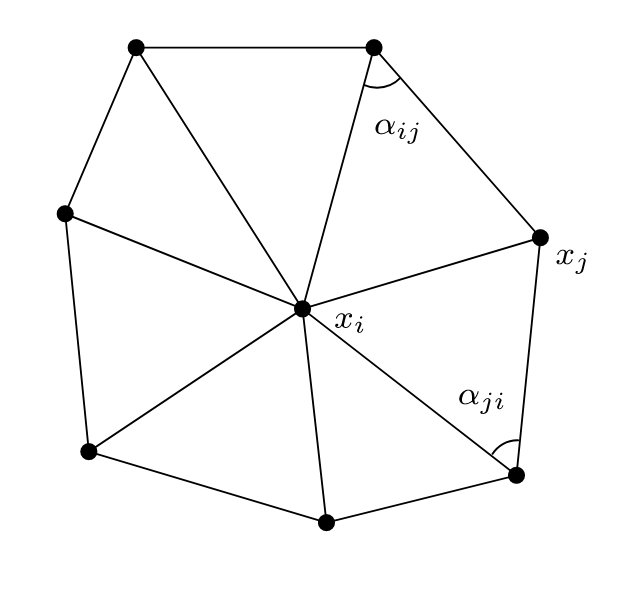
\includegraphics[width=0.4\linewidth]{resources/img/cotangent_approx.png}
	\caption{Berechnung der $\alpha$-Winkel für eine innere Kante~\cite{laplace_beltrami_paper}.}
	\label{fig:cotangent_approx}
\end{figure}

\begin{equation}
    \label{eq:cotangent_weight}
    v(x_i,x_j) = 
        \begin{cases}
            \cot{\alpha_{ij}}+\cot{\alpha_{ji}}\ & \text{for interior edges} \\
            \cot{\alpha_{ij}} & \text{for boundary edges}
        \end{cases}
\end{equation}

Aus den Kotangens-Gewichten aus Gleichung~\ref{eq:cotangent_weight} kann nun in Formel~\ref{eq:laplace_beltrami} der Laplace-Beltrami Operator in seiner Matrix-Form berechnet werden \cite{spd_solver_paper,laplace_beltrami_paper}. Dabei bescheibt $N(x_i)$ die Menge der benachbarten Vertices von $x_i$. Da für das Lösen der Gleichung~\ref{eq:bone_heat} lediglich die Matrix $(-\Delta+\textbf{H})$ benötigt wird, kann diese in der Implementierung direkt als eine Matrix erstellt werden. Die Normalisierungsfaktoren aus~\cite{spd_solver_paper} wurden hier weggelassen, da sie für diese Anwendung sowieso wegfallen.

\begin{equation}
    \label{eq:laplace_beltrami}
    \Delta_{ij}=
    \begin{cases}
        0 & i \neq j, x_j \notin N(x_i) \\
        v(x_i,x_j) & i \neq j, x_j \in N(x_i) \\
        -\sum_{x_j\in N(v_i)} v(x_i,x_j) & i = j\\
    \end{cases}
\end{equation}

Da die Matrix $\textbf{H}$ eine Diagonalmatrix ist und der Operator $\Delta$ eines Vertex durch seine direkten Nachbarn lokal definiert ist, ist die zu lösende Matrix extrem dünn besetzt. Durch die Euler-Charakteristik für Dreiecks-Netze ergeben sich nur ungefähr $7$ Einträge in der Matrix pro Reihe~\cite{spd_solver_paper}. Ein solches System lässt sich, wie in~\cite{spd_solver_paper} gezeigt, sehr effizient lösen, wenn es sich um eine SPD-Matrix (symetrisch positiv definit) handelt. Die Matrix ist durch die Konstruktion symetrisch. (TODO Delaunay Bedingung erklären und Verbindung zu Definitheit erklären)